%Usually an article, 12pt font, with a seperate title page
\documentclass[12pt,titlepage]{article}
%Ability to include figures easily, and eps files
\usepackage{graphicx}
\usepackage{grffile}
\usepackage{epstopdf}
\usepackage{epsfig}
\usepackage[euler]{textgreek}
%Hide links on autoref, and call each piece a section
\usepackage[hidelinks]{hyperref}
\def\subsectionautorefname{Section}
\def\subsubsectionautorefname{Section}
%Allows symbols, captions, math
\usepackage{amssymb}
% \usepackage{amsmath} %can also use to align equations
\usepackage{caption}
%Allow acronyms, with the list beneath
\usepackage[nolist,nohyperlinks]{acronym}
\begin{acronym}
\end{acronym}
%Use natbib for bibliography
\usepackage[square,super,comma,sort&compress]{natbib}
%Style changes, indent all paragraphs, use the full page size, change the section heads, nice fractions, nice tables
\usepackage{indentfirst}
\usepackage[margin=1in]{geometry}
\usepackage{setspace}
\onehalfspacing
\usepackage[small]{titlesec}
\titlelabel{\thetitle. }
\usepackage{nicefrac}
\usepackage{booktabs}
\newcommand\tab[1][1cm]{\hspace*{#1}}
%Allows for me to non-justify some regions
\usepackage{ragged2e}

% Another package for doing title of assignment --> got it from Joel
%\usepackage{titlesec}
%\titleformat{\subsection}[runin]
%{\normalfont\large\bfseries}{\thesubsection}{1em}{}
%\titleformat{\subsubsection}[runin]
%{\normalfont\normalsize\bfseries}{\thesubsubsection}{1em}{}
\usepackage{pdflscape}
\usepackage{enumitem}% http://ctan.org/pkg/enumitem
\usepackage{adjustbox}



\begin{document}

\begin{titlepage}

\newcommand{\HRule}{\rule{\linewidth}{0.5mm}} % Defines a new command for the horizontal lines, change thickness here

\center % Center everything on the page
 
%	HEADING SECTIONS

\textsc{\LARGE McMaster University}\\[1.5cm] % Name of your university/college
\textsc{\Large MECHTRON 4TB6A}\\[0.5cm] % Major heading such as course name
\textsc{\large Mechatronics \& Software Engineering Capstone}\\[0.5cm] % Minor heading such as course title

%	TITLE SECTION
\vspace{1cm}
\HRule \\[0.2cm]
{ \Large \vspace{0.25cm}  \textsc{  \LARGE System Design } \vspace{0.3cm} }  % Title of your document
\HRule \vspace{1cm}

\textsc{\LARGE Pill Dispenser}
 
 \begin{figure}[h]
  \centering
  
\includegraphics[width=.4\linewidth]{../ApexEngineering.png}
\end{figure}
 \vspace{1cm}
 
%----------------------------------------------------------------------------------------
%	AUTHOR SECTION
%----------------------------------------------------------------------------------------

\begin{table}[ht!]
\centering
\begin{tabular}{c c c}
\toprule
\textbf{Name} & \textbf{Student Number} & \textbf{McMaster Email}         \\ \midrule
Justin Ballaro & 400015482 & ballaroj@mcmaster.ca \\
Joel Bates & 001420696 & batesjj@mcmaster.ca \\
Brodie Bresette & 400029059 & bresettb@mcmaster.ca \\
Nicholas D'Angelo & 400018631 &  dangelon@mcmaster.ca  \\
Daniel Pietrangelo & 400010287 &  pietrand@mcmaster.ca \\
  \bottomrule
\end{tabular}
\label{Tab:HU}
\end{table}

%	DATE SECTION
\vfill
{\large Sunday, January 17, 2021}\\[3cm] % Date, change the \today to a set date if you want to be precise
 % Fill the rest of the page with whitespace

\end{titlepage}

\pagebreak
\pagenumbering{roman}
\tableofcontents
\listoffigures
\pagebreak
\listoftables
\pagebreak
\pagenumbering{arabic}

\section{Table of Revisions}

\begin{table}[ht!]
\begin{center}
\begin{adjustbox}{max width=\textwidth}
\small
\begin{tabular}{|p{0.1\textwidth}|p{0.2\textwidth}|p{0.2\textwidth}|p{0.4\textwidth}|}
 \hline
 \textbf{Revision } & \textbf{Date} &
 \textbf{Authors} &
 \textbf{Revision Comments}\\
 \hline \centering
 0 & \centering
 01/17/2021 & 
 Justin Ballaro \newline
Joel Bates \newline
Brodie Bresette \newline
Nicholas D'Angelo \newline
Daniel Pietrangelo &
Initial Revision \\
\hline
\end{tabular}
\end{adjustbox}
\end{center}
\caption{Table of Revisions}
\end{table}

\pagebreak

\section{Introduction}
\subsection{Purpose of Document}
The purpose of this document is to outline the system design. This system design was based on the declared system requirements. This outline will include a general overview of the of all system components included in the current design.

\subsection{System Scope}
The system to be implemented will provide real time alarms/reminders when it is time for the user to take their medication. The system will also dispense the user's medication in such a manor as to make it easy to retrieve and ingest from the inserted medication pouches/sachets. Once a scheduled dose has been taken/missed the system will record adherence data. This data will be stored locally on the device.\\

This project's scope consists of four main components.
\begin{enumerate}
    \item System to insert sachets into the device.
    \item System for dispensing individual medication sachets.
    \item Embedded control system that initiates dispensing, reads manual commands, and collects data.
    \item User interface for user information and settings control.
\end{enumerate}

\pagebreak
\section{System Overview}
\subsection{System Context}

 \begin{figure}[!htbp]
  \centering
  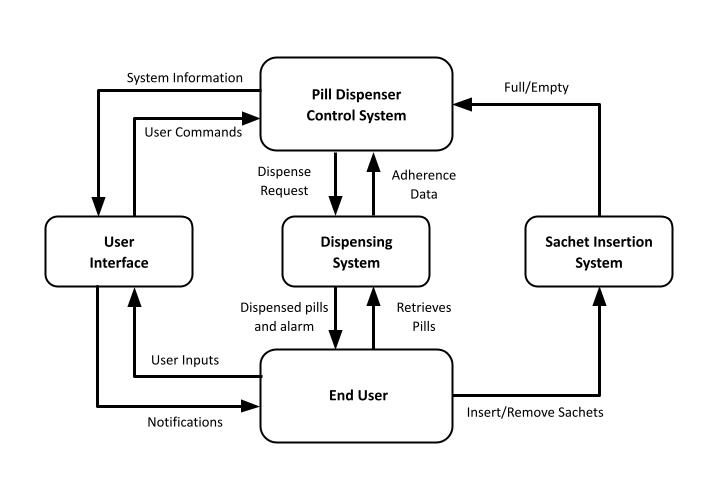
\includegraphics[width=1\linewidth]{ContextDiagram.jpg}
  \caption{Context Diagram}
\end{figure}
\pagebreak

% \subsection{Scheduling System}
% This system allows the user to set a dispensing time for each dispensing period (Morning, Afternoon, Evening, Night).
% \subsection{Notification System}
% The device's notification system will alert the user when the time has been reached to take their scheduled medication. This includes an audible alarm, along with other measures yet to be defined.
% \subsection{Loading System}
% This system will allow the user to load the desired strip pack sachet into the device.
% \subsection{Calibration System}
% The calibration system will ensure the strip pack sachets are loaded properly into the device, all system parameters are set correctly and the dispensing mechanism is in working order. 
% \subsection{Dispensing System}
% The dispensing system for the device will perform the required motion to successfully deliver the sachets allowing the pills to be retrieved from the dispensing area. This system also includes the mechanism for pill retrieval.
% \subsection{Data Collection System}
% Data collection for the device will involve collecting on-board sensor data to retrieve metrics on medication adherence and device use. 

\begin{landscape}
\subsection{Diagram of Components}


  \begin{figure}[htbp!]
  \centering
  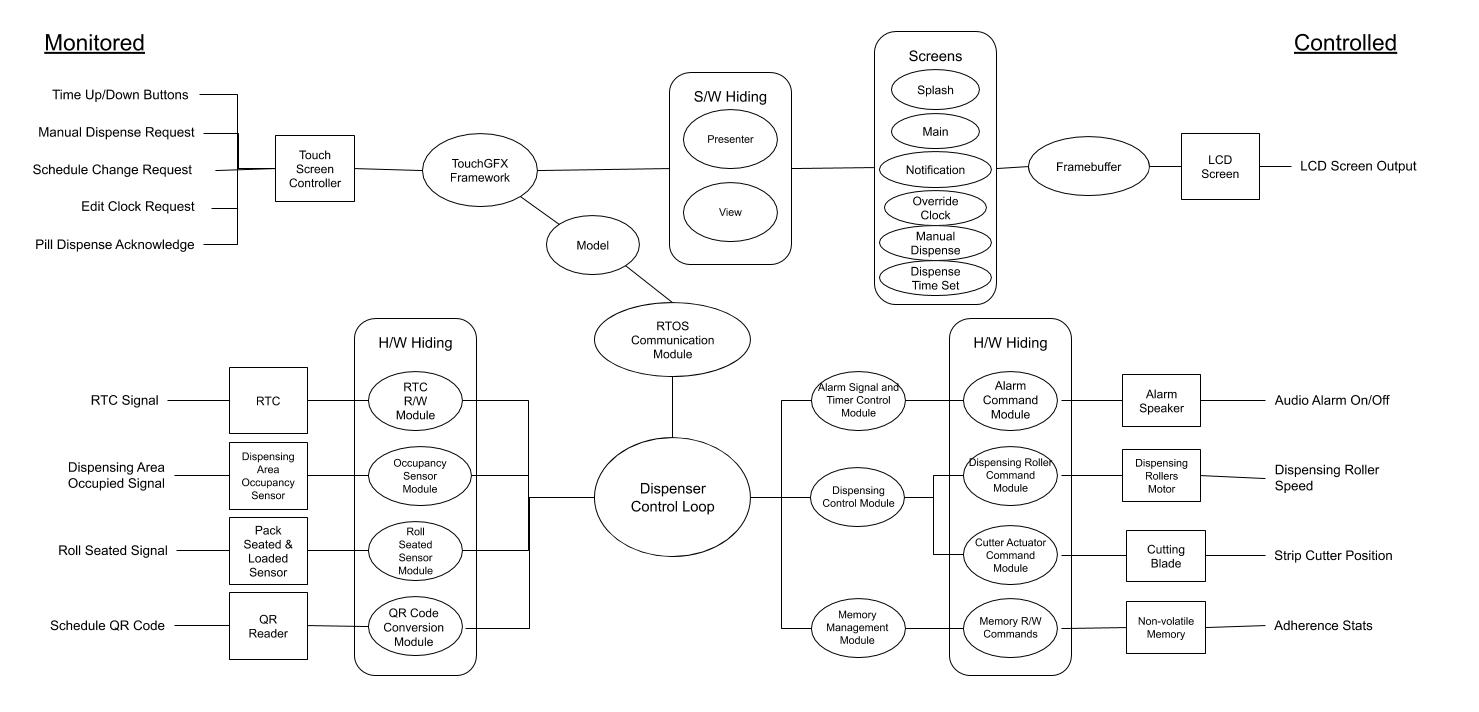
\includegraphics[width=\linewidth]{ComponentDiagram.jpg}
  \caption{Component Diagram}
\end{figure}


\pagebreak
\end{landscape}

\subsection{Monitored Variables}
\begin{table}[!htbp]
\begin{center}
\begin{adjustbox}{max width=\textwidth}
\small
\begin{tabular}{|p{0.3\textwidth}|p{0.5\textwidth}|p{0.10\textwidth}|}
 \hline
 \textbf{Name} & \textbf{Description} & \textbf{Units}\\
 \hline 
RTC Signal & Needed to follow medication schedule. & dd:mm:yy\\
 \hline
Dispensing Area \newline Occupied Signal & Whether or not a pill sachet is sitting in the dispensing area. & bool\\
 \hline
 Roll Seated Signal & Keeps track of whether or not the roll of pill sachets is within the device and seated properly. & bool\\
 \hline
  Schedule QR Code & QR code on sachet that contains schedule for dispensing time. & json \newline csv \\
 \hline
Manual Dispense Request & Button/command used to manually dispense medication. & bool \\
  \hline
  Schedule Change Request & Button/command used to request an edit to the dispensing schedule. & bool \\
  \hline
    Edit Clock Request & Button/command used to request an edit to the displayed clock. & bool \\
  \hline
   Time up/Down Buttons & Buttons used to edit schedule and clock time (up and down). & bool \\
  \hline
  Pill Dispense Acknowledgement & Button pushed to exit alarm or alarm timeout state, initiates pill dispensing protocol. & bool \\
  \hline

\end{tabular}
\end{adjustbox}
\end{center}
\caption{Monitored variables.}
\end{table}

\subsection{Controlled Variables}
\begin{table}[!htbp]
\begin{center}
\begin{adjustbox}{max width=\textwidth}
\small
\begin{tabular}{|p{0.3\textwidth}|p{0.5\textwidth}|p{0.10\textwidth}|}
 \hline
 \textbf{Name} & \textbf{Description} & \textbf{Units}\\
 \hline 
Audio Alarm On/Off & Signal to turn on and off alarm system. & bool\\
 \hline
Dispensing Roller Speed & Speed of the rollers which dispense the pill sachets. & rpm\\
 \hline
Strip Cutter Position & Distance traveled by cutting head actuator. & cm\\
 \hline
 Adherence Stats & R/W of adherence data from non-volatile memory. & json\\
 \hline
  LCD Screen Output & Content displayed on the LCD touchscreen UI. & N/A\\
 \hline 

\end{tabular}
\end{adjustbox}
\end{center}
\caption{Controlled Variables.}
\end{table}

\pagebreak

\subsection{Constants}

\begin{table}[ht!]
\begin{center}
\begin{adjustbox}{max width=\textwidth}
\small
\begin{tabular}{|p{0.6\textwidth}|p{0.5\textwidth}|p{0.10\textwidth}|}
 \hline
 \textbf{Name} & \textbf{Description} & \textbf{Units}\\
 \hline 
 Pill Dispenser Height and Width & The overall size of the Pill Dispensing machine & cm\\
 \hline
  Sachet size & Length, width and height of pouch. & cm\\
 \hline
   Sachet box & Length, width and height of pouch. & cm\\
 \hline
 Dispensing Mechanism Components & TBD & TBD \\
 \hline
\end{tabular}
\end{adjustbox}
\end{center}
\caption{Constant variables.}
\end{table}


\section{Behaviour Overview}

\begin{table}[htb!]
\begin{center}
\begin{adjustbox}{max width=.9\textwidth}
\small
\begin{tabular}{|p{0.5\textwidth}|p{0.5\textwidth}|}
 \hline
 \textbf{Required Behaviour} & \textbf{Rationale} \\
 \hline
 The system should know that the sachets are inserted correctly before dispensing can occur.  & The system must know that the pill sachets are inserted and seated correctly so that pills my be dispensed accurately, and damage to the machine may be avoided.\\
 \hline 
 The system should dispense the correct sachet at the correct time or time period based on a given schedule with 99.9\% accuracy. &
%  \begin{itemize}
%      \item The system shall store the given schedule locally after it is uploaded/inputted into the device.
%  \end{itemize} &

 Dispensing the incorrect sachet at a time not defined by the schedule can cause confusion for the user and potential health complications.\\
 \hline
 The system should notify the user when it is time to take their medication in accordance with the programmed schedule.
   &  An audible and visual alarm is necessary to notify the user when it is time to take their medication. These reminders are necessary to aid to user in pill adherence and to notify them when it is time to interact with the device.
 \\
 \hline
 The system should know what sachet is being dispensed. &
 The system should store this detail for use in adherence statistics. This should also allow the system to keep track of dispensing statistics.\\
 \hline
 The system must collect and store data on pill schedule adherence. & 
 Having these statistics available for the end user will give new insight into their health.\\
 \hline
 The system should be safe and easy to operate for all users. &
 The device should not become an extra nuisance or unsafe for the health professional or end user. \\
 \hline
 The system must not damage any pills in the dispensing process. &
 If a pill is damaged in any step of the dispensing process, it becomes unusable and the patients medication schedule is put in jeopardy.\\
 \hline
  The system must notify the user when the inserted sachet roll is nearly empty and entirely empty. & This behaviour is necessary as to let the user know that it is time to replace the currently loaded sachet roll with a new one.\\
  \hline
 
\end{tabular}
\end{adjustbox}
\end{center}
\caption{Behaviour Description Table}
\end{table}

\pagebreak

\section{Module Traceability}

This will be added in a future revision.

\section {Module Overview - UI}

\subsection{MID \& MIS}

For UI design, the TouchGFX graphic design framework created by STM was used. This framework provides generated code based on the designed UI using their 'Designer' software. The code generated from the Designer software follows a 'Model, Presenter, View' workflow. This generated code can then be altered as need to add custom functionality based on UI events (button clicks, etc).

An overview of the Model, Presenter and View workflow can be seen in Figure 3. A more detailed explanation can be found in the STM TouchGFX Documentation, found \textbf{\href{https://support.touchgfx.com/docs/development/ui-development/software-architecture/model-view-presenter-design-pattern/}{here}}

 \begin{figure}[!htbp]
  \centering
  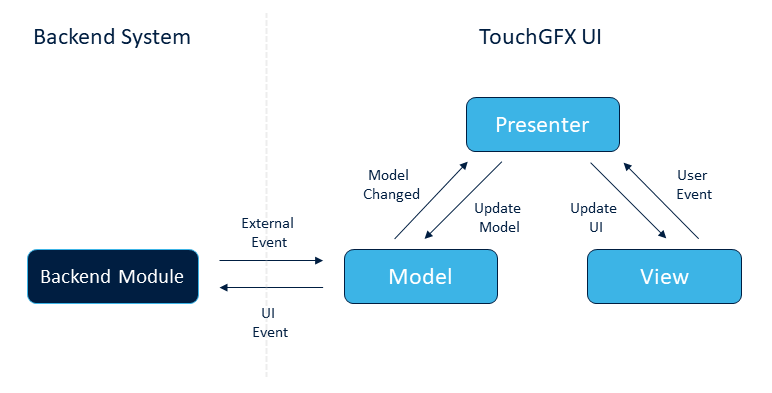
\includegraphics[width=.7\linewidth]{MVP.png}
  \caption{Model, Presenter, View workflow}
\end{figure}

The diagram of components outlines the following modules as UI components consisting of a Presenter and View:

\begin{itemize}
    \item Splash
    \item Main
    \item Notification
    \item Override Clock
    \item Manual Dispense
    \item Set Dispense Time
\end{itemize}

Custom functionality must be added to the generated View and Presenter files created for these modules. Therefore, a MID and MIS will be outlined for each. These outlines will only include any custom variables and methods defined that are needed for the custom functionality and will omit the methods created by TouchGFX as they are common amongst all View and Presenter modules. These common methods and variables can be found in the general MIS of the View and Presenter modules.

After the required UI modules are created, TouchGFX takes care of writing the required bytes to the framebuffer for rendering to the LCD screen.

\subsubsection{Module: Model}
\subsubsection*{MIS}

\noindent An outline of the Model functionality can be found in the STM Documentation found \textbf{\href{https://support.touchgfx.com/docs/development/ui-development/software-architecture/screen-definition-and-mvp/#model}{here}}. \\

\noindent \textbf{Interface} \\

\noindent \textbf{Uses}

\noindent All Presenter modules present. \\

\noindent \textbf{Variables}

\noindent Variables of this module cannot be provided at this time. Once the module is complete, the variable types will be added accordingly. \\

\noindent \textbf{Methods}

\noindent The access methods are a WIP and will be updated accordingly at a later revision.

\textit{get\_notification}


Returns whether to display a notification and what information to include.

\textit{get\_dispense\_times}

Returns the currently set dispense times.

\textit{get\_clock}

Returns current RTC value to be displayed.

\textit{set\_man\_req}

Sets request for manual dispense.

\textit{set\_notif}

Sets state of notification.

\subsubsection*{MID}

\noindent \textbf{Implementation} 

\noindent The implementations below are a WIP and will be updated accordingly at a later revision.\\

\noindent \textbf{Variables}

TBD \\

\noindent \textbf{Access Methods} \par

\textit{get\_notification} \par
Inputs: None \par
Outputs: std::string& \textit{\_notif} \par
Updates: None  \newline

\textit{get\_dispense\_times} \par
Inputs: None \par
Outputs: std::string& \textit{\_disp\_times} \par
Updates: None \newline

\textit{get\_clock} \par
Inputs: None \par
Outputs: std::string& \textit{\_time} \par
Updates: None \newline

\textit{set\_man\_req} \par
Inputs: bool \textit{should\_disp} \par
Outputs: bool \textit{\_dispensed} \par
Updates: None \newline

\textit{set\_notif} \par
Inputs: std::string& \textit{notif\_state} \par
Outputs: None \par
Updates: None \newline


\subsubsection{Module: Presenter}
\subsubsection*{MIS}

\noindent An outline of the Presenter functionality can be found in the STM Documentation found \textbf{\href{https://support.touchgfx.com/docs/development/ui-development/software-architecture/screen-definition-and-mvp/#model}{here}}. \\

\noindent \textbf{Interface} \\

\noindent \textbf{Uses}

\noindent All View modules present will each reference its own Presenter. \\

\noindent \textbf{Variables}

\noindent None \\

\noindent \textbf{Methods}

\textit{activate} \par
The activate function is called automatically when a screen transition causes this Presenter to become active. Initialization code for the presenter will be placed here

\textit{deactivate} \par
The deactivate function is called automatically when a screen transition causes this Presenter to become inactive. Cleanup code for the Presenter will be placed here.

\subsubsection{Module: View}
\subsubsection*{MIS}

\noindent An outline of the View functionality can be found in the STM Documentation found \textbf{\href{https://support.touchgfx.com/docs/development/ui-development/software-architecture/screen-definition-and-mvp/#model}{here}}. \\

\noindent \textbf{Interface} \\

\noindent \textbf{Uses}

\noindent All View modules present will each reference its own Presenter. \\

\noindent \textbf{Variables}

\noindent None \\

\noindent \textbf{Access Methods}

\textit{setupScreen} \par
The activate function is called automatically when a screen transition causes this View to become active. Initialization code for the View will be placed here

\textit{tearDownScreen} \par
The deactivate function is called automatically when a screen transition causes this View to become inactive. Cleanup code for the View will be placed here.


\subsubsection{Module: Splash}
\subsubsection*{MIS}

\noindent The Splash module will display a image on the device LCD as the device powers on. 

\noindent \textbf{Interface} \\

\noindent \textbf{Uses}

\noindent LCD Content Module \\

\noindent \textbf{Public Variables}

\noindent \textit{\_background} : \textit{touchgfx::Box} \newline
\noindent \textit{\_logo} : \textit{touchgfx::Image} \newline

\noindent \textbf{Access Methods}

\noindent The access methods are a WIP and will be updated accordingly at a later revision.

\subsubsection*{MID}

\noindent \textbf{Implementation} 

\noindent The implementations below are a WIP and will be updated accordingly at a later revision.\\

\noindent \textbf{Variables}

touchgfx::Box \_background; \par
touchgfx::Image \_logo; \newline

\noindent \textbf{Access Methods} 

TBD

\subsubsection{Module: Main}
\subsubsection*{MIS}

\noindent The Main module will display a general overview of information when the device is in a 'waiting' state. The module will display the current time, along with information regarding the next scheduled dispensing time and access to other components of the user interface. \\

\noindent \textbf{Interface} \\

\noindent \textbf{Uses}

\noindent LCD Content Module \\

\noindent \textbf{Variables}

\noindent The variables for this module are still a WIP and will be updated at a later revision. \newline

\noindent \textit{\_background} : \textit{touchgfx::Box} \newline
\noindent \textit{\_clock} : \textit{touchgfx::TextArea} \newline
\noindent \textit{\_next\_disp\_text} : \textit{touchgfx::TextArea} \newline

\noindent \textbf{Access Methods}

\noindent The access methods are a WIP and will be updated accordingly at a later revision.

\subsubsection*{MID}

\noindent \textbf{Implementation} 

\noindent The implementations below are a WIP and will be updated accordingly at a later revision.\\

\noindent \textbf{Variables}

touchgfx::Box \_background; \par
touchgfx::TextArea \_clock; \par
touchgfx::TextArea \_next\_disp\_text; \newline

\noindent \textbf{Access Methods} 

TBD


\subsubsection{Module: Notification}
\subsubsection*{MIS}

\noindent The Notification module will display a information and alert the user when a dispensing time has been reached. This module will also allow the user to trigger the dispensing action through a button click.  \\

\noindent \textbf{Interface} \\

\noindent \textbf{Uses}

\noindent LCD Content Module \\

\noindent \textbf{Variables}

\noindent The variables for this module are still a WIP and will be updated at a later revision. \newline

\noindent \textit{\_background} : \textit{touchgfx::Box} \newline
\noindent \textit{\_dispense\_button} : \textit{touchgfx::Button} \newline

\noindent \textbf{Access Methods}

\noindent The access methods are a WIP and will be updated accordingly at a later revision. \par

\textit{buttonCallbackHandler} \par
Catches button click and will invoke functionality from set\_notification.

\textit{set\_notification} \par
Send request to model to set current notification to 'dismiss'

\subsubsection*{MID}

\noindent \textbf{Implementation} 

\noindent The implementations below are a WIP and will be updated accordingly at a later revision.\\

\noindent \textbf{Variables}

touchgfx::Box \_background; \par
touchgfx::Button \_dispense\_button; \newline

\noindent \textbf{Access Methods} 

\textit{buttonCallbackHandler} \par
Inputs: const touchgfx::AbstractButton& \textit{src} \par
Outputs: None \par
Updates: None \newline

\textit{set\_notification} \par
Inputs: std::string& \textit{notif\_state} \par
Outputs: None \par
Updates: None \newline



\subsubsection{Module: OverrideClock}
\subsubsection*{MIS}

\noindent The OverrideClock module will allow the user to update the current onboard time.  \\

\noindent \textbf{Interface} \\

\noindent \textbf{Uses}

\noindent LCD Content Module \\

\noindent \textbf{Variables}

\noindent The variables for this module are still a WIP and will be updated at a later revision. \newline

\noindent \textit{\_background} : \textit{touchgfx::Box} \newline
\noindent \textit{\_new\_clock} : \textit{touchgfx::TextArea} \newline
\noindent \textit{\_inc\_button} : \textit{touchgfx::Button} \newline
\noindent \textit{\_dec\_button} : \textit{touchgfx::Button} \newline

\noindent \textbf{Access Methods}

\noindent The access methods are a WIP and will be updated accordingly at a later revision. \par

\textit{buttonCallbackHandler1} \par
Catches inc button click and will invoke inc\_time functionality.

\textit{buttonCallbackHandler2} \par
Catches dec button click and will invoke dec\_time functionality.

\textit{inc\_time} \par
Increase time.

\textit{dec\_time} \par
Decrease time.

\textit{set\_time} \par
Sends request to set time for board.

\subsubsection*{MID}

\noindent \textbf{Implementation} 

\noindent The implementations below are a WIP and will be updated accordingly at a later revision.\\

\noindent \textbf{Variables}

touchgfx::Box \_background; \par
touchgfx::TextArea \_new\_clock; \par
touchgfx::Button \_inc\_button; \par
touchgfx::Button \_dec\_button; \newline

\noindent \textbf{Access Methods} 

\textit{buttonCallbackHandle1} \par
Inputs: const touchgfx::AbstractButton& \textit{src} \par
Outputs: None \par
Updates: None \newline

\textit{buttonCallbackHandle2} \par
Inputs: const touchgfx::AbstractButton& \textit{src} \par
Outputs: None \par
Updates: None \newline

\textit{set\_time} \par
Inputs: None \par
Outputs: None \par
Updates: None \newline

\textit{inc\_time} \par
Inputs: None \par
Outputs: None \par
Updates: None \newline

Will set appropriate area in \_new\_clock text area. \newline

\textit{dec\_time} \par
Inputs: None \par
Outputs: None \par
Updates: None \newline

Will set appropriate area in \_new\_clock text area.

\textit{set\_time} \par
Inputs: std::string& \textit{time} \par
Outputs: None \par
Updates: None \newline


\subsubsection{Module: ManualDispense}
\subsubsection*{MIS}

\noindent The ManualDispense module will allow the user to request dispensing outside the defined dispensing times.  \\

\noindent \textbf{Interface} \\

\noindent \textbf{Uses}

\noindent LCD Content Module \\

\noindent \textbf{Variables}

\noindent The variables for this module are still a WIP and will be updated at a later revision. \newline

\noindent \textit{\_background} : \textit{touchgfx::Box} \newline
\noindent \textit{\_disp\_now\_button} : \textit{touchgfx::Button} \newline

\noindent \textbf{Access Methods}

\noindent The access methods are a WIP and will be updated accordingly at a later revision. \par

\textit{buttonCallbackHandler} \par
Catches inc button click and will invoke inc\_time functionality.

\textit{set\_man\_request} \par
Sends request to model for manual dispense request.

\subsubsection*{MID}

\noindent \textbf{Implementation} 

\noindent The implementations below are a WIP and will be updated accordingly at a later revision.\\

\noindent \textbf{Variables}

touchgfx::Box \_background; \par
touchgfx::Button \_disp\_now\_button; \par

\noindent \textbf{Access Methods} 

\textit{buttonCallbackHandle} \par
Inputs: const touchgfx::AbstractButton& \textit{src} \par
Outputs: None \par
Updates: None \newline

\textit{set\_man\_request} \par
Inputs: bool \textit{req} \par
Outputs: None \par
Updates: None \newline



\subsubsection{Module: SetDispenseTime}
\subsubsection*{MIS}

\noindent The SetDispenseTime module will allow the user to change the currently set dispensing time.  \\

\noindent \textbf{Interface} \\

\noindent \textbf{Uses}

\noindent LCD Content Module \\

\noindent \textbf{Variables}

\noindent The variables for this module are still a WIP and will be updated at a later revision. \par

\noindent \textit{\_background} : \textit{touchgfx::Box} \newline
\noindent \textit{\_current\_disp\_time} : \textit{touchgfx::ScrollList} \newline
\noindent \textit{\_selected\_disp\_time\_text} : \textit{touchgfx::TextArea} \newline
\noindent \textit{\_selected\_disp\_time} : \textit{std::string} \newline
\noindent \textit{\_inc\_button} : \textit{touchgfx::Button} \newline
\noindent \textit{\_dec\_button} : \textit{touchgfx::Button} \newline


\noindent \textbf{Access Methods}

\noindent The access methods are a WIP and will be updated accordingly at a later revision. \par

\textit{buttonCallbackHandler1} \par
Catches inc button click and will invoke inc\_time functionality.

\textit{buttonCallbackHandler2} \par
Catches dec button click and will invoke dec\_time functionality.

\textit{buttonCallbackHandler3} \par
Catches set button click and will invoke dec\_time functionality.

\textit{sel\_disp\_time} \par
Select dispense time to change.

\textit{inc\_time} \par
Increase time.

\textit{dec\_time} \par
Decrease time.

\textit{set\_time} \par
Sends request to set time for board.

\subsubsection*{MID}

\noindent \textbf{Implementation} 

\noindent The implementations below are a WIP and will be updated accordingly at a later revision.\\

\noindent \textbf{Variables}

touchgfx::Box \_background; \par
touchgfx::ScrollList \_current\_disp\_time; \par
touchgfx::TextArea \_selected\_disp\_time\_text \par
std::string touchgfx::TextArea \_selected\_disp\_time \par
touchgfx::Button \_inc\_button; \par
touchgfx::Button \_dec\_button; \par
touchgfx::Button \_set\_button; \newline

\noindent \textbf{Access Methods} 

\textit{buttonCallbackHandle1} \par
Inputs: const touchgfx::AbstractButton& \textit{src} \par
Outputs: None \par
Updates: None \newline

\textit{buttonCallbackHandle2} \par
Inputs: const touchgfx::AbstractButton& \textit{src} \par
Outputs: None \par
Updates: None \newline

\textit{buttonCallbackHandle3} \par
Inputs: const touchgfx::AbstractButton& \textit{src} \par
Outputs: None \par
Updates: None \newline

\textit{set\_time} \par
Inputs: None \par
Outputs: None \par
Updates: None \newline

\textit{inc\_time} \par
Inputs: None \par
Outputs: None \par
Updates: None \newline

Will set appropriate area in \_new\_clock text area. \newline

\textit{dec\_time} \par
Inputs: None \par
Outputs: None \par
Updates: None \newline

Will set appropriate area in \_new\_clock text area. \newline

\textit{sel\_disp\_time} \par
Inputs: std::string& \textit{time} \par
Outputs: None \par
Updates: \_selected\_disp\_time \newline





\pagebreak
\section{Component Overview}
\subsection{RTC Hardware}
\subsubsection*{Description}
Off the shelf real time clock powered by a battery, to allow for time to be kept accurately even in the case of a power outage. 
\subsubsection*{Inputs and Outputs}

\begin{table}[ht!]
\begin{center}
\begin{adjustbox}{max width=\textwidth}
\small
\begin{tabular}{|p{0.2\textwidth}|p{0.2\textwidth}|p{0.10\textwidth}|p{0.1\textwidth}|p{0.4\textwidth}|}
 \hline
 \textbf{Input Name} & \textbf{Input Type} & \textbf{Units} &\textbf{Range} & \textbf{Comments} \\
 \hline 
MCUclkInput & Analog square wave & Voltage & 0-5V & Allows for serial communication to be synchronized between MCU and RTC\\
 \hline 
MCUtimeReq & hexadecimal address & hex & 00h-12h & These addresses return specific date information and can also be used to set time.\\
 \hline
\end{tabular}
\end{adjustbox}
\end{center}
\caption{RTC Hardware Inputs}
\end{table}

\begin{table}[ht!]
\begin{center}
\begin{adjustbox}{max width=\textwidth}
\small
\begin{tabular}{|p{0.2\textwidth}|p{0.2\textwidth}|p{0.10\textwidth}|p{0.1\textwidth}|p{0.4\textwidth}|}
 \hline
 \textbf{Output Name} & \textbf{Output Type} & \textbf{Units} &\textbf{Range} & \textbf{Comments} \\
 \hline 
 RTCclockSignal & 8 bit & int & 0 or 1 & Clock output is an 8 bit number transmitted over serial through an I2C bidirectional bus \\
 \hline
\end{tabular}
\end{adjustbox}
\end{center}
\caption{RTC Hardware Outputs}
\end{table}

\subsubsection*{Timing Constraints}
Chosen chip uses a 400kHz I2C interface and there is a 350ns delay as the that is the amount of time required for the chip to register the request. 

\subsubsection*{Initialization}
Using the two input pins a start signal must be sent to the RTC. 

\subsection{Dispensing Area Occupancy Sensor}
\subsubsection*{Description}
This component will sense whether a pill sachet has successfully been dispensed by the device and when it is removed.
\subsubsection*{Inputs and Outputs}

\begin{table}[ht!]
\begin{center}
\begin{adjustbox}{max width=\textwidth}
\small
\begin{tabular}{|p{0.2\textwidth}|p{0.2\textwidth}|p{0.10\textwidth}|p{0.1\textwidth}|p{0.4\textwidth}|}
 \hline
 \textbf{Input Name} & \textbf{Input Type} & \textbf{Units} &\textbf{Range} & \textbf{Comments} \\
 \hline 
 N/A & N/A  & N/A & N/A & N/A \\
 \hline
\end{tabular}
\end{adjustbox}
\end{center}
\caption{Dispensing Area Occupancy Sensor Inputs}
\end{table}

\begin{table}[ht!]
\begin{center}
\begin{adjustbox}{max width=\textwidth}
\small
\begin{tabular}{|p{0.2\textwidth}|p{0.2\textwidth}|p{0.10\textwidth}|p{0.1\textwidth}|p{0.4\textwidth}|}
 \hline
 \textbf{Output Name} & \textbf{Output Type} & \textbf{Units} &\textbf{Range} & \textbf{Comments} \\
 \hline 
 dispensingAreaFull & Boolean & N/A & 0/1 & N/A \\
 \hline
\end{tabular}
\end{adjustbox}
\end{center}
\caption{Dispensing Area Occupancy Sensor Outputs}
\end{table}

\subsubsection*{Timing Constraints}
The sensor for the dispensing area should be checking at least every 0.5s to see if there is something in the area.
\subsubsection*{Initialization}
The dispensingAreaFull output should be initialized to 0 and then respond to the sensor.
\subsection{Pill Roll Sensor}
\subsubsection*{Description}
This component will determine if the pill sachet container has been correctly input into the device.
\subsubsection*{Inputs and Outputs}

\begin{table}[ht!]
\begin{center}
\begin{adjustbox}{max width=\textwidth}
\small
\begin{tabular}{|p{0.2\textwidth}|p{0.2\textwidth}|p{0.10\textwidth}|p{0.1\textwidth}|p{0.4\textwidth}|}
 \hline
 \textbf{Input Name} & \textbf{Input Type} & \textbf{Units} &\textbf{Range} & \textbf{Comments} \\
 \hline 
 N/A & N/A  & N/A & N/A & N/A \\
 \hline
\end{tabular}
\end{adjustbox}
\end{center}
\caption{Pill Roll Seated Sensor Inputs}
\end{table}

\begin{table}[ht!]
\begin{center}
\begin{adjustbox}{max width=\textwidth}
\small
\begin{tabular}{|p{0.2\textwidth}|p{0.2\textwidth}|p{0.10\textwidth}|p{0.1\textwidth}|p{0.4\textwidth}|}
 \hline
 \textbf{Output Name} & \textbf{Output Type} & \textbf{Units} &\textbf{Range} & \textbf{Comments} \\
 \hline 
  pillRollSeated & Boolean & N/A & 0/1 & N/A \\
 \hline
\end{tabular}
\end{adjustbox}
\end{center}
\caption{Pill Roll Seated Sensor Outputs}
\end{table}
\subsubsection*{Timing Constraints}
The sensor for the pill roll should begin to monitor when it detects no pill roll in the device, whether it be as a result of the previously placed roll shifting within the device, or if the roll is being replaced. 
\subsubsection*{Initialization}
The pill roll seated sensor will initialize to 1 if the device is turned on and the pill roll is correctly placed, or 0 if there is no pill roll / the pill roll is incorrectly positioned.
\subsection{QR Reader Hardware}
\subsubsection*{Description}
Each pill sachet includes a small QR code with details regarding the specific pills included in the sachet. This QR reader will scan the QR code on the sachet and provide the relevant information attained from scanning.
\subsubsection*{Inputs and Outputs}

\begin{table}[ht!]
\begin{center}
\begin{adjustbox}{max width=\textwidth}
\small
\begin{tabular}{|p{0.2\textwidth}|p{0.2\textwidth}|p{0.10\textwidth}|p{0.1\textwidth}|p{0.4\textwidth}|}
 \hline
 \textbf{Input Name} & \textbf{Input Type} & \textbf{Units} &\textbf{Range} & \textbf{Comments} \\
 \hline 
 startQRscan & Boolean & N/A & 0/1 & N/A \\
 \hline
\end{tabular}
\end{adjustbox}
\end{center}
\caption{QR Reader Hardware Inputs}
\end{table}

\begin{table}[ht!]
\begin{center}
\begin{adjustbox}{max width=\textwidth}
\small
\begin{tabular}{|p{0.2\textwidth}|p{0.2\textwidth}|p{0.10\textwidth}|p{0.1\textwidth}|p{0.4\textwidth}|}
 \hline
 \textbf{Output Name} & \textbf{Output Type} & \textbf{Units} &\textbf{Range} & \textbf{Comments} \\
 \hline 
 QRcodeData & String & char[] & N/A & N/A \\
 \hline
\end{tabular}
\end{adjustbox}
\end{center}
\caption{QR Reader Hardware Outputs}
\end{table}

\subsubsection*{Timing Constraints}
The QR code reader should be able to successfully read an individual pill sachet QR code within 5 seconds.
\subsubsection*{Initialization}
The QR code reader will be initialized to 0 and only change once having successfully read a QR code.
\subsection{Touch Screen Controller Hardware}
\subsubsection*{Description}
This component is a touch-enabled LCD screen that will allow the user to interact with the pill dispensing device. A variety of on-display buttons will send requests to the UI framework (touchGFX) to enter the corresponding screen.
\subsubsection*{Inputs and Outputs}

\begin{table}[ht!]
\begin{center}
\begin{adjustbox}{max width=\textwidth}
\small
\begin{tabular}{|p{0.3\textwidth}|p{0.2\textwidth}|p{0.10\textwidth}|p{0.1\textwidth}|p{0.4\textwidth}|}
 \hline
 \textbf{Input Name} & \textbf{Input Type} & \textbf{Units} &\textbf{Range} & \textbf{Comments} \\
 \hline 
 buttonUpDown & Boolean & N/A & 0/1 & N/A \\
 \hline
 manualDispenseRequest & Boolean & N/A & 0/1 & N/A \\
 \hline
 pillTimeChangeRequest & Boolean & N/A & 0/1 & N/A \\
 \hline
 editClockRequest & Boolean & N/A & 0/1 & N/A \\
 \hline
 dispenseAcknowledgement & Boolean & N/A & 0/1 & N/A \\
 \hline
\end{tabular}
\end{adjustbox}
\end{center}
\caption{Touch Screen Controller Hardware Inputs}
\end{table}

\begin{table}[ht!]
\begin{center}
\begin{adjustbox}{max width=\textwidth}
\small
\begin{tabular}{|p{0.2\textwidth}|p{0.2\textwidth}|p{0.10\textwidth}|p{0.1\textwidth}|p{0.4\textwidth}|}
 \hline
 \textbf{Output Name} & \textbf{Output Type} & \textbf{Units} &\textbf{Range} & \textbf{Comments} \\
 \hline 
 N/A & N/A & N/A & N/A & N/A \\
 \hline
\end{tabular}
\end{adjustbox}
\end{center}
\caption{Touch Screen Controller Hardware Outputs}
\end{table}

\subsubsection*{Timing Constraints}
Successful button presses on the LCD screen should cause changes in the UI in real-time.
\subsubsection*{Initialization}
The LCD screen will be initialized to the home display.

\subsection{RTC Module}
\subsubsection*{Description}
Take the signal from the RTC hardware and output the date and time from it to the MCU. As well as allowing MCU to set date and time on the RTC.
\subsubsection*{Inputs and Outputs}
$ $\\
\begin{table}[ht!]
\begin{center}
\begin{adjustbox}{max width=\textwidth}
\small
\begin{tabular}{|p{0.2\textwidth}|p{0.2\textwidth}|p{0.10\textwidth}|p{0.1\textwidth}|p{0.4\textwidth}|}
 \hline
 \textbf{Input Name} & \textbf{Input Type} & \textbf{Units} &\textbf{Range} & \textbf{Comments} \\
 \hline 
 RTCclockSignal  & 8 bit  & int & 0 or 1 & Clock output is an 8 bit number transmitted over serial through an I2C bidirectional bus \\
 \hline
  getTime  &  boolean & N/A & true or false & Input from MCU asking for time \\
 \hline
 writeTime  & DateTime  & yr:mm:dd hr:min:sec & 0:0:0 0:0:0 to 9999:12:31 23:59:59 & Time to write to RTC sent from MCU \\
 \hline
\end{tabular}
\end{adjustbox}
\end{center}
\caption{RTC Module Inputs}
\end{table}
  \\

\begin{table}[ht!]
\begin{center}
\begin{adjustbox}{max width=\textwidth}
\small
\begin{tabular}{|p{0.2\textwidth}|p{0.2\textwidth}|p{0.10\textwidth}|p{0.1\textwidth}|p{0.4\textwidth}|}
 \hline
 \textbf{Output Name} & \textbf{Output Type} & \textbf{Units} &\textbf{Range} & \textbf{Comments} \\
 \hline 
 RTCtime & DateTime  & yr:mm:dd hr:min:sec & 0:0:0 0:0:0 to 9999:12:31 23:59:59 & Time to write to MCU \\
 \hline
 MCUtime & 8 bit  & int & 0 or 1 & Time to write for MCU to RTC \\
 \hline
 RTCaddress & hexadecimal  & N/A & 00h-12h & Address to write new time into on RTC \\
 \hline
\end{tabular}
\end{adjustbox}
\end{center}
\caption{RTC Module Outputs}
\end{table}
\subsubsection*{Timing Constraints}
This must be done within 100ms to ensure loss of time is insignificant to end user
\subsubsection*{Initialization}
This module initializes by sending the start command to the RTC. 

\subsection{Occupancy Sensor Module}
\subsubsection*{Description}
Take information from the dispensing area occupancy sensor to debounce and do any other necessary operations to ensure a clean sensor output. 
\subsubsection*{Inputs and Outputs}

\begin{table}[ht!]
\begin{center}
\begin{adjustbox}{max width=\textwidth}
\small
\begin{tabular}{|p{0.2\textwidth}|p{0.2\textwidth}|p{0.10\textwidth}|p{0.1\textwidth}|p{0.4\textwidth}|}
 \hline
 \textbf{Input Name} & \textbf{Input Type} & \textbf{Units} &\textbf{Range} & \textbf{Comments} \\
 \hline 
 dispensingAreaFull & Boolean  & N/A & 0/1 & N/A \\
 \hline
\end{tabular}
\end{adjustbox}
\end{center}
\caption{Occupancy Sensor Module Inputs}
\end{table}

\begin{table}[ht!]
\begin{center}
\begin{adjustbox}{max width=\textwidth}
\small
\begin{tabular}{|p{0.25\textwidth}|p{0.2\textwidth}|p{0.10\textwidth}|p{0.1\textwidth}|p{0.35\textwidth}|}
 \hline
 \textbf{Output Name} & \textbf{Output Type} & \textbf{Units} &\textbf{Range} & \textbf{Comments} \\
 \hline 
 dispensingAreaFullDB & Boolean & N/A & 0/1 & Debounced sensor output \\
 \hline
\end{tabular}
\end{adjustbox}
\end{center}
\caption{Occupancy Sensor Module Outputs}
\end{table}

\subsubsection*{Timing Constraints}
This Module should respond within 0.5 seconds.
\subsubsection*{Initialization}
The output of this should be initialized to 0 and then respond to the sensor.

\subsection{Pill Roll Sensor Module}
\subsubsection*{Description}
This module will take the sensor input and determine if the roll is correctly seated, this will be output to the MCU.
\subsubsection*{Inputs and Outputs}
$ $\\
\begin{table}[ht!]
\begin{center}
\begin{adjustbox}{max width=\textwidth}
\small
\begin{tabular}{|p{0.2\textwidth}|p{0.2\textwidth}|p{0.10\textwidth}|p{0.1\textwidth}|p{0.4\textwidth}|}
 \hline
 \textbf{Input Name} & \textbf{Input Type} & \textbf{Units} &\textbf{Range} & \textbf{Comments} \\
 \hline 
 RollsensorInput & boolean  & N/A & True/False & Raw sensor input from the digital output of the sensor. \\
 \hline
\end{tabular}
\end{adjustbox}
\end{center}
\caption{Pill Roll Sensor Module Inputs}
\end{table}

\begin{table}[ht!]
\begin{center}
\begin{adjustbox}{max width=\textwidth}
\small
\begin{tabular}{|p{0.2\textwidth}|p{0.2\textwidth}|p{0.10\textwidth}|p{0.1\textwidth}|p{0.4\textwidth}|}
 \hline
 \textbf{Output Name} & \textbf{Output Type} & \textbf{Units} &\textbf{Range} & \textbf{Comments} \\
 \hline 
 Rollseated & boolean & N/A & True/False & True if roll is seated correct, false otherwise. \\
 \hline
\end{tabular}
\end{adjustbox}
\end{center}
\caption{Pill Roll Sensor Module Outputs}
\end{table}

\subsubsection*{Timing Constraints}
this will need to have a reliable output from the sensor data within 250ms of the sensor changing to ensure proper functionality.
\subsubsection*{Initialization}
On initialization the default value for the Rollseated variable would be false.

\subsection{QR Code Conversion Module}
\subsubsection*{Description}
This module takes in the raw QR scanner output and formats it to be used in the Dispenser Control module. 
\subsubsection*{Inputs and Outputs}
\begin{table}[ht!]
\begin{center}
\begin{adjustbox}{max width=\textwidth}
\small
\begin{tabular}{|p{0.2\textwidth}|p{0.2\textwidth}|p{0.10\textwidth}|p{0.1\textwidth}|p{0.4\textwidth}|}
 \hline
 \textbf{Input Name} & \textbf{Input Type} & \textbf{Units} &\textbf{Range} & \textbf{Comments} \\
 \hline 
 QRcodeData & String & char[] & N/A & Raw string output from QR code reader \\
 \hline
 startQRscanIn & Boolean & N/A & 0/1 & Input from control loop to get QR reading. \\
 \hline
\end{tabular}
\end{adjustbox}
\end{center}
\caption{QR Code Conversion Module Inputs}
\end{table}

\begin{table}[ht!]
\begin{center}
\begin{adjustbox}{max width=\textwidth}
\small
\begin{tabular}{|p{0.2\textwidth}|p{0.2\textwidth}|p{0.10\textwidth}|p{0.1\textwidth}|p{0.4\textwidth}|}
 \hline
 \textbf{Output Name} & \textbf{Output Type} & \textbf{Units} &\textbf{Range} & \textbf{Comments} \\
 \hline 
 QRcodeFormatted & String & char[] & N/A & Formatted QR code data for use in control loop \\
 \hline
 startQRscanOut & Boolean & N/A & 0/1 & passed from control loop to the QR hardware \\
 \hline
\end{tabular}
\end{adjustbox}
\end{center}
\caption{QR Code Conversion Module Outputs}
\end{table}

\subsubsection*{Timing Constraints}
The formatting of the string should have very little effect on timing. Formatting should be completed on the order of 1ms. 
\subsubsection*{Initialization}
On initialization the output string should be null. 

\subsection{Dispenser Control Module}
\subsubsection*{Description}
The control loop responsible for initiating control functions for device operation. This component keeps track of the current state as well as conditions necessary to move between states.

\subsubsection*{Inputs and Outputs}

\begin{table}[ht!]
\begin{center}
\begin{adjustbox}{max width=\textwidth}
\small
\begin{tabular}{|p{0.3\textwidth}|p{0.1\textwidth}|p{0.10\textwidth}|p{0.1\textwidth}|p{0.4\textwidth}|}
 \hline
 \textbf{Input Name} & \textbf{Input Type} & \textbf{Units} &\textbf{Range} & \textbf{Comments} \\
 \hline 
 RTOSMessage & TBD  & TBD & TBD & Messages received from RTOS control module. \\
 \hline
 RTCTime & DateTime  & yr:mm:dd \newline hr:min:sec & 0:0:0 \newline 0:0:0 to \newline 9999:12:31 \newline 23:59:59 & Time received from RTC. \\
 \hline
 RTOSMessage & TBD  & TBD & TBD & Messages received from RTOS control module. \\
 \hline
 DispenseRequest & Boolean  & N/A & 0/1 & Request to dispense next pill sachet. \\
 \hline
 isDispenseAreaOccupied & Boolean  & N/A & 0/1 & Whether or not a sachet is in the dispensing area. \\
 \hline
  AdherenceUpdateResponse & Boolean  & N/A & 0/1 & Whether or not an adherence data update was successful or not. \\
 \hline
\end{tabular}
\end{adjustbox}
\end{center}

\caption{Dispenser Control Module Inputs}
\end{table}

\begin{table}[ht!]
\begin{center}
\begin{adjustbox}{max width=\textwidth}
\small
\begin{tabular}{|p{0.3\textwidth}|p{0.1\textwidth}|p{0.10\textwidth}|p{0.1\textwidth}|p{0.4\textwidth}|}
 \hline
 \textbf{Output Name} & \textbf{Output Type} & \textbf{Units} &\textbf{Range} & \textbf{Comments} \\
 \hline 
 InitiateDispense & Boolean & N/A & 0/1 & Initiates the dispensing protocol. \\
 \hline
 AlarmOnOff & Boolean & N/A & 0/1 & Activates and deactivates audible alarm system. \\
 \hline
  WriteAdherence & Boolean & N/A & 0/1 & Submits request to update adherence data based on latest dispensing event. \\
 \hline
UpdateRequest & TBD & TBD & TBD & Update request sent as RTOS message. Includes schedule and RTC updates. \\
 \hline
\end{tabular}
\end{adjustbox}
\end{center}
\caption{Dispenser Control Module Outputs}
\end{table}

\subsubsection*{Timing Constraints}
All signals received or sent by the control loop must be read/written within 1-2 milliseconds. 

\subsubsection*{Initialization}
The control loop module is initialized in the INIT state. Within this state a system calibration is performed. The control loop will not move to the next state until it is deemed safe to do so.

\pagebreak

\subsubsection*{Control Flow Diagram}

 \begin{figure}[ht!]
  \centering
  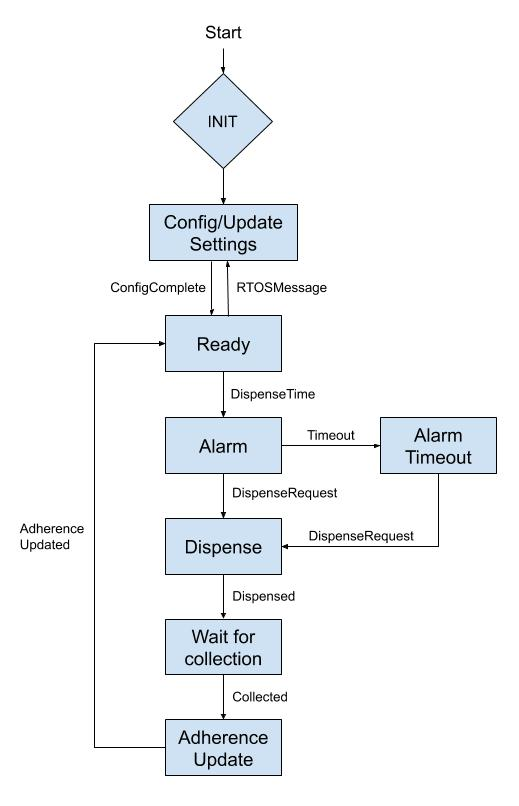
\includegraphics[width=.7\linewidth]{system_design/Dispenser FSM.jpg}
  \caption{Control Loop Flow Chart}
\end{figure}

\pagebreak

\subsubsection*{State Description}
\begin{enumerate}
    \item Config/Update Settings - In this state the control loop looks at update requests from the RTOS and proceeds to make the appropriate updates. Upon completion of all updates the loop proceeds to the ready state.
    \item Ready - In this state the control loop waits for the current time to match that of the next scheduled dose. When this occurs a transition to the Alarm state takes place. In the ready state the loop also looks for update requests from the RTOS.
    \item Alarm - In this state the system proceeds to turn on the audible alarm. This alarm will continue until a DispenseRequest is received or until the timeout limit has been reached.
    \item Alarm Timeout - In this state the audible alarm is shut off and the system waits for a DispenseRequest input to proceed.
    \item Dispense - In this state the control loop initiates the sachet dispensing process. When a sachet has been dispensed the system proceeds to the wait for collection state.
    \item Wait for Collection - In this state the control loop monitors the occupancy of the dispensing area. Once the dispense sachet has been collected the system proceeds to update adherence data.
    \item Adherence Update - In this state the control loop initiates the adherence data update process. The system proceeds back to the ready state once a message signaling a successful data update has been received.
\end{enumerate}

%\subsection{LCD Content Module}
%\subsubsection*{Description}
%\subsubsection*{Inputs and Outputs}

%\begin{table}[ht!]
%\begin{center}
%\begin{adjustbox}{max width=\textwidth}
%\small
%\begin{tabular}{|p{0.2\textwidth}|p{0.2\textwidth}|p{0.10\textwidth}|%p{0.1\textwidth}|p{0.4\textwidth}|}
% \hline
% \textbf{Input Name} & \textbf{Input Type} & \textbf{Units} %&\textbf{Range} & \textbf{Comments} \\
% \hline 
% Input & Input Type  & Units & Range & Comments \\
% \hline
% Input & Input Type  & Units & Range & Comments \\
% \hline
%\end{tabular}
%\end{adjustbox}
%\end{center}
%\caption{LCD Content Module Inputs}
%\end{table}

%\begin{table}[ht!]
%\begin{center}
%\begin{adjustbox}{max width=\textwidth}
%\small
%begin{tabular}{|p{0.2\textwidth}|p{0.2\textwidth}|p{0.10\textwidth}|p%{0.1\textwidth}|p{0.4\textwidth}|}
% \hline
% \textbf{Output Name} & \textbf{Output Type} & \textbf{Units} %&\textbf{Range} & \textbf{Comments} \\
% \hline 
% Output & Output Type & Units & Range & Comments \\
% \hline
% Output & Output Type & Units & Range & Comments \\
% \hline
%\end{tabular}
%\end{adjustbox}
%\end{center}
%\caption{LCD Content Module Outputs}
%\end{table}

%\subsubsection*{Timing Constraints}
%\subsubsection*{Initialization}

\subsection{RTOS Communication Module}
\subsubsection*{Description}

The RTOS Communication Module allows for interprocess communication between the GUI and Dispenser Control Loop. This communication will allows updates to flow from both sources.
\pagebreak

\subsubsection*{Inputs and Outputs}

\begin{table}[htbp!]
\begin{center}
\begin{adjustbox}{max width=\textwidth}
\small
\begin{tabular}{|p{0.2\textwidth}|p{0.2\textwidth}|p{0.10\textwidth}|p{0.1\textwidth}|p{0.4\textwidth}|}
 \hline
 \textbf{Input Name} & \textbf{Input Type} & \textbf{Units} &\textbf{Range} & \textbf{Comments} \\
 \hline 
 guiQueue & xQueueHandle  & N/A & N/A & GUI task message queue \\
 \hline
 FSMQueue & xQueueHandle  & N/A & N/A & FSM task message queue \\
 \hline
 msg & uint8\_t  & N/A & N/A & Messages to be added to queue \\
 \hline
\end{tabular}
\end{adjustbox}
\end{center}
\caption{RTOS Communication Module Inputs}
\end{table}

\begin{table}[ht!]
\begin{center}
\begin{adjustbox}{max width=\textwidth}
\small
\begin{tabular}{|p{0.2\textwidth}|p{0.2\textwidth}|p{0.10\textwidth}|p{0.1\textwidth}|p{0.4\textwidth}|}
 \hline
 \textbf{Output Name} & \textbf{Output Type} & \textbf{Units} &\textbf{Range} & \textbf{Comments} \\
 \hline 
 N/A & N/A & N/A & N/A & N/A \\
 \hline
\end{tabular}
\end{adjustbox}
\end{center}
\caption{RTOS Communication Module Outputs}
\end{table}

%\subsubsection*{Timing Constraints}
%\subsubsection*{Initialization}


\subsection{Alarm and Timer Module }
\subsubsection*{Description}
This module sets the alarm to be active from the control loop.
\subsubsection*{Inputs and Outputs}

\begin{table}[ht!]
\begin{center}
\begin{adjustbox}{max width=\textwidth}
\small
\begin{tabular}{|p{0.2\textwidth}|p{0.2\textwidth}|p{0.10\textwidth}|p{0.1\textwidth}|p{0.4\textwidth}|}
 \hline
 \textbf{Input Name} & \textbf{Input Type} & \textbf{Units} &\textbf{Range} & \textbf{Comments} \\
 \hline 
 alarmActive & Boolean  & N/A & 0/1 & N/A \\
 \hline
\end{tabular}
\end{adjustbox}
\end{center}
\caption{Alarm and Timer Module Inputs}
\end{table}

\begin{table}[ht!]
\begin{center}
\begin{adjustbox}{max width=\textwidth}
\small
\begin{tabular}{|p{0.2\textwidth}|p{0.2\textwidth}|p{0.10\textwidth}|p{0.1\textwidth}|p{0.4\textwidth}|}
 \hline
 \textbf{Output Name} & \textbf{Output Type} & \textbf{Units} &\textbf{Range} & \textbf{Comments} \\
 \hline 
 alarmSpeaker & Boolean & N/A & 0/1 & N/A \\
 \hline
\end{tabular}
\end{adjustbox}
\end{center}
\caption{Alarm and Timer Module Outputs}
\end{table}

\subsubsection*{Timing Constraints}
The alarm module should respond within 1 second of receiving its signal.
\subsubsection*{Initialization}
The alarm inputs and outputs should be initialized to 0.
\subsection{Dispensing Roller Command Module }
\subsubsection*{Description}
This module controls the stepper motor(s) used to dispense a sachet.
\subsubsection*{Inputs and Outputs}

\begin{table}[ht!]
\begin{center}
\begin{adjustbox}{max width=\textwidth}
\small
\begin{tabular}{|p{0.2\textwidth}|p{0.2\textwidth}|p{0.10\textwidth}|p{0.1\textwidth}|p{0.4\textwidth}|}
 \hline
 \textbf{Input Name} & \textbf{Input Type} & \textbf{Units} &\textbf{Range} & \textbf{Comments} \\
 \hline 
 startDispense & Boolean  & N/A & 0/1 & N/A \\
 \hline
\end{tabular}
\end{adjustbox}
\end{center}
\caption{Dispensing Roller Command Module Inputs}
\end{table}

\begin{table}[ht!]
\begin{center}
\begin{adjustbox}{max width=\textwidth}
\small
\begin{tabular}{|p{0.2\textwidth}|p{0.2\textwidth}|p{0.10\textwidth}|p{0.1\textwidth}|p{0.4\textwidth}|}
 \hline
 \textbf{Output Name} & \textbf{Output Type} & \textbf{Units} &\textbf{Range} & \textbf{Comments} \\
 \hline 
 StepperMotorIn & Square Wave & Volts & 0-5 & N/A \\
 \hline
\end{tabular}
\end{adjustbox}
\end{center}
\caption{Dispensing Roller Command Module Outputs}
\end{table}

%\subsubsection*{Timing Constraints}
%\subsubsection*{Initialization}

\subsection{Cutting Actuator Command Module }
\subsubsection*{Description}
This module will take input from the control loop and send and output to the cutting actuator to cut open pill sachets.
\subsubsection*{Inputs and Outputs}
 
\begin{table}[ht!]
\begin{center}
\begin{adjustbox}{max width=\textwidth}
\small
\begin{tabular}{|p{0.2\textwidth}|p{0.2\textwidth}|p{0.10\textwidth}|p{0.1\textwidth}|p{0.4\textwidth}|}
 \hline
 \textbf{Input Name} & \textbf{Input Type} & \textbf{Units} &\textbf{Range} & \textbf{Comments} \\
 \hline 
 cuttingActuatorIn & Boolean  & N/A & 0/1 & N/A \\
 \hline
\end{tabular}
\end{adjustbox}
\end{center}
\caption{Cutting Actuator Command Module Inputs}
\end{table}

\begin{table}[ht!]
\begin{center}
\begin{adjustbox}{max width=\textwidth}
\small
\begin{tabular}{|p{0.2\textwidth}|p{0.2\textwidth}|p{0.10\textwidth}|p{0.1\textwidth}|p{0.4\textwidth}|}
 \hline
 \textbf{Output Name} & \textbf{Output Type} & \textbf{Units} &\textbf{Range} & \textbf{Comments} \\
 \hline 
 linearCutter & Boolean & N/A & 0/1 & N/A \\
 \hline
\end{tabular}
\end{adjustbox}
\end{center}
\caption{Cutting Actuator Command Module Outputs}
\end{table}

% \subsubsection*{Timing Constraints}
% \subsubsection*{Initialization}


\subsection{Alarm Speaker Hardware }
\subsubsection*{Description}
The alarm speaker will go off when the schedule says it is time for the user to take their next medication.
\subsubsection*{Inputs and Outputs}

\begin{table}[ht!]
\begin{center}
\begin{adjustbox}{max width=\textwidth}
\small
\begin{tabular}{|p{0.2\textwidth}|p{0.2\textwidth}|p{0.10\textwidth}|p{0.1\textwidth}|p{0.4\textwidth}|}
 \hline
 \textbf{Input Name} & \textbf{Input Type} & \textbf{Units} &\textbf{Range} & \textbf{Comments} \\
 \hline 
 alarmSpeaker & Boolean  & N/A & 0/1 & 1-Alarm is on; 0-Alarm is off \\
 \hline
\end{tabular}
\end{adjustbox}
\end{center}
\caption{Alarm Speaker Hardware Inputs}
\end{table}

\begin{table}[ht!]
\begin{center}
\begin{adjustbox}{max width=\textwidth}
\small
\begin{tabular}{|p{0.2\textwidth}|p{0.2\textwidth}|p{0.10\textwidth}|p{0.1\textwidth}|p{0.4\textwidth}|}
 \hline
 \textbf{Output Name} & \textbf{Output Type} & \textbf{Units} &\textbf{Range} & \textbf{Comments} \\
 \hline 
 N/A & N/A & N/A & N/A & N/A \\
 \hline
\end{tabular}
\end{adjustbox}
\end{center}
\caption{Alarm Speaker Hardware Outputs}
\end{table}

\subsubsection*{Timing Constraints}
The Alarm Speaker should sound for 10 minutes once a pill sachet is ready for dispensing.  
\subsubsection*{Initialization}
The Alarm will be initialized to being off.
\subsection{Stepper Motor Roller Hardware }
\subsubsection*{Description}
Used to control the stepper motor which is used to push the pill sachets out of the device.
\subsubsection*{Inputs and Outputs}

\begin{table}[ht!]
\begin{center}
\begin{adjustbox}{max width=\textwidth}
\small
\begin{tabular}{|p{0.2\textwidth}|p{0.2\textwidth}|p{0.10\textwidth}|p{0.1\textwidth}|p{0.4\textwidth}|}
 \hline
 \textbf{Input Name} & \textbf{Input Type} & \textbf{Units} &\textbf{Range} & \textbf{Comments} \\
 \hline 
 StepperMotorIn & Square Wave & Volts & 0-5 & N/A \\
 \hline
\end{tabular}
\end{adjustbox}
\end{center}
\caption{Stepper Motor Roller Inputs}
\end{table}

\begin{table}[ht!]
\begin{center}
\begin{adjustbox}{max width=\textwidth}
\small
\begin{tabular}{|p{0.2\textwidth}|p{0.2\textwidth}|p{0.10\textwidth}|p{0.1\textwidth}|p{0.4\textwidth}|}
 \hline
 \textbf{Output Name} & \textbf{Output Type} & \textbf{Units} &\textbf{Range} & \textbf{Comments} \\
 \hline 
 N/A & N/A & N/A & N/A & N/A \\
 \hline
\end{tabular}
\end{adjustbox}
\end{center}
\caption{Stepper Motor Roller Outputs}
\end{table}

%\subsubsection*{Timing Constraints}
%\subsubsection*{Initialization}

\subsection{Linear Actuated Cutter Hardware }
\subsubsection*{Description}
The Linear Actuated Cutter is the hardware by which the individual pill sachets will be cut from the pill roll.
\subsubsection*{Inputs and Outputs}

\begin{table}[ht!]
\begin{center}
\begin{adjustbox}{max width=\textwidth}
\small
\begin{tabular}{|p{0.2\textwidth}|p{0.2\textwidth}|p{0.10\textwidth}|p{0.1\textwidth}|p{0.4\textwidth}|}
 \hline
 \textbf{Input Name} & \textbf{Input Type} & \textbf{Units} &\textbf{Range} & \textbf{Comments} \\
 \hline 
 linearCutter & Boolean & N/A & 0/1 & 1-Cut; 0-Don't cut \\
 \hline
\end{tabular}
\end{adjustbox}
\end{center}
\caption{Linear Actuated Cutter Inputs}
\end{table}

\begin{table}[ht!]
\begin{center}
\begin{adjustbox}{max width=\textwidth}
\small
\begin{tabular}{|p{0.2\textwidth}|p{0.2\textwidth}|p{0.10\textwidth}|p{0.1\textwidth}|p{0.4\textwidth}|}
 \hline
 \textbf{Output Name} & \textbf{Output Type} & \textbf{Units} &\textbf{Range} & \textbf{Comments} \\
 \hline 
 N/A & N/A & N/A & N/A & N/A \\
 \hline
\end{tabular}
\end{adjustbox}
\end{center}
\caption{Linear Actuated Cutter Outputs}
\end{table}

\subsubsection*{Timing Constraints}
Once receiving the cutting boolean input, the linear actuated cutter should respond within 5 seconds to begin the cutting motion.
\subsubsection*{Initialization}
This component is initialized to 0; a do not cut state.

\subsection{Memory Management Module }
\subsubsection*{Description}
This module manages on a high level the memory requests and facilitates read and write requests. 
\subsubsection*{Inputs and Outputs}

\begin{table}[ht!]
\begin{center}
\begin{adjustbox}{max width=\textwidth}
\small
\begin{tabular}{|p{0.2\textwidth}|p{0.2\textwidth}|p{0.10\textwidth}|p{0.1\textwidth}|p{0.4\textwidth}|}
 \hline
 \textbf{Input Name} & \textbf{Input Type} & \textbf{Units} &\textbf{Range} & \textbf{Comments} \\
 \hline 
   clkIn & square wave  & Voltage & 0-5V & Clock input in from the control module to allow for synchronous serial communication.  \\
 \hline
schedData & String  & N/A & N/A & This is schedule data passed from the control module to be written to memory chip.  \\
 \hline
 retrieveData & bool & N/A & True/False & This is a request from the control module for the current schedule data.  \\
 \hline
\end{tabular}
\end{adjustbox}
\end{center}
\caption{Memory Management Module Inputs}
\end{table}

\begin{table}[ht!]
\begin{center}
\begin{adjustbox}{max width=\textwidth}
\small
\begin{tabular}{|p{0.2\textwidth}|p{0.2\textwidth}|p{0.10\textwidth}|p{0.1\textwidth}|p{0.4\textwidth}|}
 \hline
 \textbf{Output Name} & \textbf{Output Type} & \textbf{Units} &\textbf{Range} & \textbf{Comments} \\
 \hline 
   clkOut & square wave  & Voltage & 0-5V & Passed through from control module to memory read write module. \\
 \hline
 getData & bool & N/A & True/False & This is a request from the memory management module for the current schedule data.  \\
 \hline
  writeData & String  & N/A & N/A & This is schedule data passed from the memory management module to be written to memory chip.  \\
 \hline
\end{tabular}
\end{adjustbox}
\end{center}
\caption{Memory Management Module Outputs}
\end{table}

\subsubsection*{Timing Constraints}
Memory should be able to be accessed with formatted data within 5ms.
\subsubsection*{Initialization}
This module should be initialized to all null until there is data sent from the control module.

\subsection{Memory Read/Write Module }
\subsubsection*{Description}
This module communicates serially through I2C with the memory chip to read and write stored data. It interprets the serial messages are formats it to a form for the control module to use. 
\subsubsection*{Inputs and Outputs}

\begin{table}[ht!]
\begin{center}
\begin{adjustbox}{max width=\textwidth}
\small
\begin{tabular}{|p{0.2\textwidth}|p{0.2\textwidth}|p{0.10\textwidth}|p{0.1\textwidth}|p{0.4\textwidth}|}
 \hline
 \textbf{Input Name} & \textbf{Input Type} & \textbf{Units} &\textbf{Range} & \textbf{Comments} \\
 serialIn & 8 bit  & N/A & 0/1 & A synchronous I2C serial connection where a 8 bit message is transmitted from the chip to the module. \\
 \hline
 writeData & String  & N/A & N/A & This is data passed in from the memory management module to be formatted and sent to the chip.  \\
 \hline
  readData & bool & N/A & True/False & This is a request from the memory management module for the current schedule data.  \\
 \hline
   clkInput & square wave  & Voltage & 0-5V & Allows synchronization with the mcu for the serial communication. \\
 \hline
\end{tabular}
\end{adjustbox}
\end{center}
\caption{Memory Read/Write Module Inputs}
\end{table}

\begin{table}[ht!]
\begin{center}
\begin{adjustbox}{max width=\textwidth}
\small
\begin{tabular}{|p{0.2\textwidth}|p{0.2\textwidth}|p{0.10\textwidth}|p{0.1\textwidth}|p{0.4\textwidth}|}
 \hline
 \textbf{Output Name} & \textbf{Output Type} & \textbf{Units} &\textbf{Range} & \textbf{Comments} \\
 \hline 
  clkOutput & square wave  & Voltage & 0-5V & Passed though to allow synchronization with the mcu for the serial communication. \\
 \hline
 memAddress & hexadecimal  & N/A & 00h-12h & Address for storage location on chip \\
 \hline
  serialOut & 8 bit  & N/A & 0/1 & Converted message from string to the serial communication data.  \\
 \hline  
 dataOut & string  & N/A & N/A & The formatted data to be sent to the memory module.  \\
 \hline
\end{tabular}
\end{adjustbox}
\end{center}
\caption{Memory Read/Write Module Outputs}
\end{table}

\subsubsection*{Timing Constraints}
Memory should be able to be accessed with formatted data within 5ms.
\subsubsection*{Initialization}
This module should be initialized to all null until there is data sent from the control module.
\subsection{Non-Volatile Memory Hardware }
\subsubsection*{Description}
This component maintains the memory where adherence data will be stored.
\subsubsection*{Inputs and Outputs}
$ $\\
\begin{table}[ht!]
\begin{center}
\begin{adjustbox}{max width=\textwidth}
\small
\begin{tabular}{|p{0.2\textwidth}|p{0.2\textwidth}|p{0.10\textwidth}|p{0.1\textwidth}|p{0.4\textwidth}|}
 \hline
 \textbf{Input Name} & \textbf{Input Type} & \textbf{Units} &\textbf{Range} & \textbf{Comments} \\
 \hline 
 memAddress & hexadecimal  & N/A & 00h-12h & Address for storage location on chip \\
 \hline
  clkInput & square wave  & Voltage & 0-5V & Allows synchronization with the mcu for the serial communication. \\
 \hline
 serialIn & 8 bit  & N/A & 0/1 & A synchronous I2C serial connection where a 8 bit message is transmitted. \\
 \hline
\end{tabular}
\end{adjustbox}
\end{center}
\caption{Non-Volatile Memory  Inputs}
\end{table}

\begin{table}[ht!]
\begin{center}
\begin{adjustbox}{max width=\textwidth}
\small
\begin{tabular}{|p{0.2\textwidth}|p{0.2\textwidth}|p{0.10\textwidth}|p{0.1\textwidth}|p{0.4\textwidth}|}
 \hline
 \textbf{Output Name} & \textbf{Output Type} & \textbf{Units} &\textbf{Range} & \textbf{Comments} \\
 \hline 
 serialOut & 8 bit  & N/A & 0/1 & A synchronous I2C serial connection where a 8 bit message is transmitted. \\
 \hline
\end{tabular}
\end{adjustbox}
\end{center}
\caption{Non-Volatile Memory  Outputs}
\end{table}
$ $\\
\subsubsection*{Timing Constraints}
The clock on this chip can run at 50MHz so it should have no meaningful timing effect.
\subsubsection*{Initialization}
The memory is initialized to be empty, but will continue to store data as pills are dispensed and taken by the patient.

\section{Normal Operation}
The strip pill dispensing device should correctly dispense pills at their scheduled times. Correctly dispensing pills entails not damaging the pills themselves, while also not dispensing too many pills. The device will sound an alarm each time a pill is ready for dispensing and will continue to ring until addressed. The UI is an LCD-touch screen that should be simple and effective, allowing the user to change the time, manually dispense pills within a reasonable amount of time when compared to the scheduled dispensing, as well as change the scheduled timing for pills.
\section{Undesired Event Handling}
The safety of the pill dispensing machine is of critical importance. As such, the device must be able to account for any number of undesired events and have thoughtful, user-friendly remediation. Below is a list of undesired events that may occur and their potential remediation. The included events have been deemed as the most likely to occur.
\subsection{Pill Dispenser Jam}
The system should be able to determine if it has jammed, attempt to fix itself, and if unsuccessful, inform the user how to return the device to a functioning state.
\subsection{Power Outage}
The system should be able to account for a power outage, returning to its previous state, and resuming operation once re-powered.
\subsection{Failed Alarm/Reminder}
The system should be able to detect if the alarming mechanisms are malfunctioning and should inform the user how to return the device to a functioning state.
\subsection{Data Transfer Error}
The system should be able to determine whether a data transfer error occurred when being programmed by the pharmacist, inform the programmer of the error and prompt the pharmacist to retry the data download.
\subsection{Pill Not Taken}
The system should be able to detect whether a pill was not taken by the user and determine whether the user should take the dosage or remove and replace it with the next dosage.

\end{document}